\documentclass{exercise}

\institute{Lehrstuhl für Strömungslehre und Aerodynamisches Institut}
\title{Selbstrechenübung 2}
\author{Joshua Feld, 406718}
\course{Strömungsmechanik I}
\professor{Schröder}
\semester{Sommersemester 2022}
\program{CES (Bachelor)}

\begin{document}
    \maketitle

    
    \section*{Aufgabe 1}
    
    \begin{problem}
        Ein Behälter ist mit einem Fluid der Dichte \(\rho\) gefüllt.
        Der Abfluss des Behälters (Füllhöhe \(H\)) ist durch eine Halbzylinderschale (Radius \(R\) und Tiefe \(T\)) luftdicht abgeschlossen.
        \begin{enumerate}
            \item Bestimmen Sie die vertikale Druckkraft auf die Schale anhand des Integrals über die Mantelfläche der Schale
            \[
                \vec{F}_p = \int_0^\pi \Delta p\parentheses*{\varphi}TR\begin{pmatrix}
                    \cos\varphi\\
                    0\\
                    \sin\varphi
                \end{pmatrix}\d\varphi.
            \]
            \item Welche Höhe (\(L\)) muss eine unten offene \emph{rechteckige} Schale mit der Breite \(2R\) und der Tiefe \(T\) haben, damit Sie die gleiche Druckkraft erfährt wie die Halbzylinderschale aus Teil a)?
            \item Überprüfen Sie das Ergebnis für die Halbzylinderschale (Teil a)) mit dem Prinzip von Stevin: Die Kraft auf eine beliebige Fläche \(A\) im Fluid entspricht dem Gewicht der Flüssigkeitssäule multipliziert mit der Projektionsfläche.
            \item Wie groß muss der Druck im Abfluss unterhalb der Schale sein, damit die Schale (Gewicht \(G\)) sich vom Boden löst?
        \end{enumerate}
        Gegeben: \(H, \rho, R, T, g, p_a, G\)
        
        \emph{Hinweis: \(\int\sin^2 x\d x = \frac{1}{2}\parentheses*{x - \sin x \cdot \cos x}\).}
    \end{problem}
    
    \subsection*{Lösung}
    Da die Halbzylinderschale nicht vollständig von Wasser umgeben (also nicht vollständig benetzt) ist, lässt sich das Prinzip von Archimedes nicht anwenden.
    Der Auftrieb kann deshalb nicht nach der Formel \(F_A = \rho gV\) berechnet werden.
    Das Gleiche gilt auch für Aufgaben, bei denen ein Gegenstand z.B. auf dem Grund eines Sees liegt.
    \begin{enumerate}
        \item Da nur die vertikale Druckkraft gesucht ist, wird lediglich die dritte Zeile von \(F_p\) betrachtet:
        \[
            F_{p, z} = \int_0^\pi \Delta p\parentheses*{\varphi}TR\sin\parentheses*{\varphi}\d\varphi.
        \]
        Um \(F_{p, z}\) zu berechnen, fehlt ein Ausdruck für die Druckdifferenz \(\Delta p\parentheses*{\varphi}\).
        Eine Druckbilanz in \(z\)-Richtung unter Berücksichtigung des in der Aufgabenstellung eingetragenen Koordinatensystems liefert
        \[
            \Delta p = -p_{\text{oben}} + p_{\text{unten}}.
        \]
        Der Druck auf die Schale von unten \(p_{\text{unten}}\) entspricht laut Aufgabenstellung dem Außendruck \(p_a\).
        Der Druck auf die Schale von oben ist abhängig von der Wassertiefe:
        \[
            p_{\text{oben}} = p_a + \rho g\parentheses*{H - z}.
        \]
        Um die Druckdifferenz in das Integral einsetzen zu können, muss sie in Abhängigkeit von \(\varphi\) ausgedrückt werden.
        Hierfür wird die Beziehung \(z = R\sin\parentheses*{\varphi}\) eingesetzt.
        Insgesamt ergibt sich
        \[
            \Delta p\parentheses*{\varphi} = -p_a - \rho g\parentheses*{H - R\sin\parentheses*{\varphi}} + p_a = -\rho g\parentheses*{H - R\sin\parentheses*{\varphi}}.
        \]
        Einsetzen in \(F_{p, z}\) liefert
        \begin{align*}
            F_{p, z} &= \int_0^\pi -\rho g\parentheses*{H - R\sin\parentheses*{\varphi}}TR\sin\parentheses*{\varphi}\d\varphi\\
            &= -\rho gTR\int_0^\pi \parentheses*{H\sin\parentheses*{\varphi} - R\sin^2\parentheses*{\varphi}}\d\varphi\\
            &= -\rho gTR\brackets*{-H\cos\parentheses*{\varphi} - \frac{R}{2}\sin^2\parentheses*{\varphi}}_0^\pi\\
            &= -2\rho gTR\parentheses*{H - \frac{\pi R}{4}}.
        \end{align*}
        Da \(R < H\) und \(\frac{\pi}{4} < 1\), ist \(F_{p, z} < 0\).
        Das bedeutet, die Kraft wirkt gegen die Koordinatenrichtung.
        Die Schale wird also zu Boden gedrückt.
        \item Erläuterung der Geometrie:
        \begin{center}
            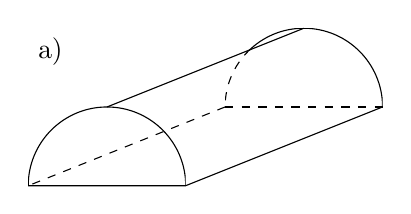
\begin{tikzpicture}
                \node[anchor=north west] at (0,2) {a)};
                \draw (0,0) -- (2,0) -- (4.5,1);
                \begin{scope}
                    \clip (0,0) rectangle (2,1);
                    \draw (1,0) circle (1cm);
                \end{scope}
                \begin{scope}
                    \clip (4.5,1) rectangle (2.8,2);
                    \draw (3.5,1) circle (1cm);
                \end{scope}
                \begin{scope}
                    \clip (2.5,1) rectangle (2.8,2);
                    \draw[dashed] (3.5,1) circle (1cm);
                \end{scope}
                \draw (3.5,2) -- (1,1);
                \draw[dashed] (2.5,1) -- (0,0);
                \draw[dashed] (2.5,1) -- (4.5,1);
            \end{tikzpicture}
            \qquad
            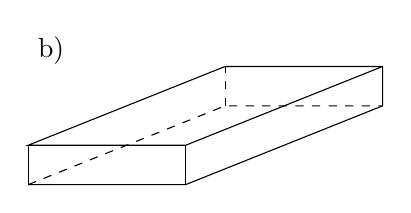
\begin{tikzpicture}
                \node[anchor=north west] at (0,2) {b)};
                \draw (0,0) -- (2,0) -- (4.5,1) -- (4.5,1.5) -- (2.5,1.5) -- (0,.5) -- (2,.5) -- (4.5,1.5);
                \draw (0,0) -- (0,.5);
                \draw (2,0) -- (2,.5);
                \draw[dashed] (0,0) -- (2.5,1) -- (4.5,1);
                \draw[dashed] (2.5,1) -- (2.5,1.5);
            \end{tikzpicture}
        \end{center}
        \[
            F_{p, z, \text{a)}} \stackrel{!}{=} F_{p, z,\text{b)}}
        \]
        \(F_{p, z, \text{b)}}\) mit Kräftegleichgewicht in \(z\)-Richtung bestimmen:
        \[
            F_{p, z, \text{b)}} = A\Delta p = 2RT\parentheses*{p_{\text{oben}, \text{b)}} + p_{\text{unten}, \text{b)}}}.
        \]
        Die Drücke betragen \(p_{\text{oben}, \text{b)}} = p_a + \rho g\parentheses*{H - L}\) und \(p_{\text{unten}, \text{b)}} = p_a\).
        Einsetzen liefert
        \[
            F_{p, z, \text{b)}} = -2RT\rho g\parentheses*{H - L}.
        \]
        Dieser Ausdruck kann nun mit \(F_{p, z, \text{a)}}\) aus a) gleichgesetzt werden:
        \[
            -2RT\rho g\parentheses*{H - L} = 2\rho gTR\parentheses*{H - \frac{\pi R}{4}} \iff L = \frac{\pi R}{4}.
        \]
        \item
        \begin{enumerate}
            \item
            \[
                \text{``Gewicht der Flüssigkeitssäule''} = \rho_W gV_{\text{Wassersäule}}.
            \]
            Das Volumen der Wassersäule ergibt sich durch Subtraktion des Halbzylindervolumens von einem Quader der Größe \(2RTH\):
            \[
                V_{\text{Wassersäule}} = 2RTH - \frac{\pi R^2 T}{2}
            \]
            \item Oberflächendruck multipliziert mit der Projektionsfläche in \(z\)-Richtung
            \begin{itemize}
                \item von unten: \(p_a \cdot 2RT = p_a A_{\text{proj}}\),
                \item von oben: \(p_a \cdot 2RT = p_a A_{\text{proj}}\).
            \end{itemize}
        \end{enumerate}
        Das Zusammensetzen der Teile (i) und (ii) mit Vorzeichen gemäß des Koordinatensystems der Aufgabenstellung liefert
        \[
            F_{p, z} = \underbrace{p_a \cdot 2RT}_{\text{Druck von unten}} - \underbrace{p_a \cdot 2RT}_{\text{Oberflächendruck auf Wasseroberfläche}} - \underbrace{\rho g\parentheses*{2RTH - \frac{\pi R^2 T}{2}}}_{\text{Gewicht des Wassers}} = F_{p, z, \text{a)}}.
        \]
        \item ``Schale löst sich'' bedeutet, dass gerade \(Gg = F_{p, z}\).
        Weil sich in \(\Delta p\parentheses*{\varphi}\) nun nicht mehr Atmosphären- und Innendruck kürzen, lautet
        \[
            F_{p, z, \text{d)}} = -2\rho gRT\parentheses*{H - \frac{\pi R}{4}} + 2RT\parentheses*{p_i - p_a}.
        \]
        Das Kräftegleichgewicht lässt sich nun wie folgt umformen:
        \[
            Gg = F_{p, z, \text{d)}} = -2\rho gRT\parentheses*{H - \frac{\pi R}{4}} + 2RT\parentheses*{p_i - p_a} \iff p_i = p_a + \frac{Gg}{2RT} + \rho g\parentheses*{H - \frac{\pi R}{4}}.
        \]
    \end{enumerate}
\end{document}
